\section{Torque observes one flux projection}
\label{sec:torque-observability}
\subsection{The question answered by a torque observation}
Reciprocity tests whether two flux surfaces can be slopes of one landscape.
It does not fix the height or all slopes of that landscape. An independent
mechanical observation poses a different question: which part of a local
flux vector contributes to electromagnetic torque? Under the amplitude-invariant
fundamental dq convention used here, the familiar relation is
\begin{equation}
 M_{\rm map}=\kt(\psid i_q-\psiq i_d),\qquad k_{\rm T}=\tfrac32p .
 \label{eq:torque-flux}
\end{equation}
The same convention must apply to both currents and fluxes
\cite{binder2017,schroeder2021,jebai2014}. With power-invariant scaling of
both vectors the coefficient is instead $p$. A scaling change cannot be
applied to just one channel. In a loss-aware model one must also specify
which currents and fluxes enter the torque law; terminal samples are not
automatically storage coordinates.

Torque-assisted parameter identification is already used for SPMSMs;
Wang et al.\ combine torque and voltage information in a sensorless
parameter estimator \cite{wang2026torque}. Here the object is an arbitrary
nonlinear flux field and its observable directions, rather than a particular
parameter estimator. The following projection is an algebraic reformulation
of \cref{eq:torque-flux}, not a claim of an established new flux species.

For nonzero stator current introduce the unit current direction and its
clockwise normal:
\begin{equation}
 \statorcurrent=\begin{bmatrix}i_d\\i_q\end{bmatrix},\quad
 \statorcurrentmagnitude=\sqrt{i_d^2+i_q^2},\quad
 \currentunitdirection=\frac{\statorcurrent}{I_s},\quad
 \torqueunitdirection=\frac{-\rotationgenerator\statorcurrent}{I_s}
                    =\frac{1}{I_s}\begin{bmatrix}i_q\\-i_d\end{bmatrix}.
 \label{eq:torque-directions}
\end{equation}
The two unit directions are orthogonal. Decomposing the flux vector gives
\begin{equation}
 \flux=\currentparallelflux\currentunitdirection+
       \torqueobservableflux\torqueunitdirection,\qquad
 \psi_i=\vect n_i\trans\flux,\quad
 \psi_\tau=\vect n_\tau\trans\flux,\quad
 M_{\rm map}=k_{\rm T}I_s\psi_\tau .
 \label{eq:torque-projection}
\end{equation}
We refer to $\psi_\tau$ as the torque-observable flux component in the
following. It is a signed, current-dependent projection in Wb, not the
flux magnitude or a separate winding linkage. Torque is the oriented
area spanned by current and flux times $k_{\rm T}$: a parallel addition
changes no area, whereas a normal addition changes it directly.
\begin{figure}[tbp]
 \centering
 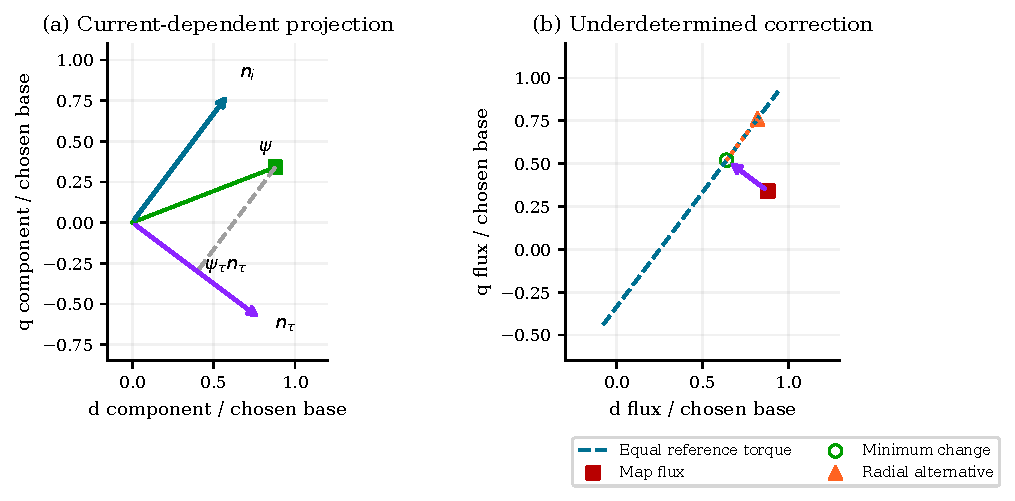
\includegraphics[width=\textwidth]{figures/06_torque_geometry.pdf}
 \caption{Local torque geometry in dimensionless coordinates. Left: a
 clockwise normal extracts the torque-producing projection; the dashed
 projection line is parallel to current. Right: a reference torque defines
 a line of admissible flux vectors. The arrow selects the closest vector;
 the triangular point adds an equally admissible radial change. Marker
 shapes and line patterns retain the distinction without color.}
 \label{fig:torque-geometry}
\end{figure}

For a qualified reference for the electromagnetic torque represented by
this model, define
\begin{equation}
 \psi_{\tau,\rm ref}=\frac{\electromagnetictorquereference}{k_{\rm T}I_s},
 \quad \torqueconsistencyresidual=M_{\rm map}-M_{\rm em,ref},
 \quad \torquefluxresidual=\psi_{\tau,\rm map}-\psi_{\tau,\rm ref}
                         =\frac{e_M}{k_{\rm T}I_s}.
 \label{eq:torque-residual}
\end{equation}
The normalized residual has flux units and compares the same observable
direction across current magnitudes. It does not attribute disagreement
to flux alone. If current is treated as exact and torque noise has standard
deviation $\sigma_M$, its contribution has
$\sigma_{\psi_\tau}=\sigma_M/(|k_{\rm T}|I_s)$. At zero current torque is
zero for every finite flux vector, the local rank becomes zero, and the
unit directions and normalized residual are undefined. A current threshold
must replace normalization near the origin, rather than an artificial
denominator epsilon.

\subsection{Rank, the solution line, and a minimum-change representative}
At fixed nonzero current, the torque row has only one scalar output:
\begin{equation}
 \vect a=-\matr J\vect i_s,\qquad
 \vect a\trans\Delta\flux=b,\qquad
 b=\frac{M_{\rm em,ref}-M_{\rm map}}{k_{\rm T}} .
 \label{eq:torque-row}
\end{equation}
Here $\vect a$ has units A and $b$ has units Wb A.
The row has rank one and kernel $\operatorname{span}\{\vect i_s\}$.
Consequently the full set of locally torque-compatible changes is
\begin{equation}
 \Delta\flux=-e_{\psi_\tau}\vect n_\tau+\alpha\vect i_s,\qquad
 \alpha\in\mathbb R .
 \label{eq:torque-family}
\end{equation}
The coefficient $\alpha$ has inductance units. An observation fixes the
normal coordinate of a line, leaving its radial coordinate free.
Minimizing Euclidean change selects the perpendicular projection onto
that line:
\begin{equation}
 \boxed{\Delta\flux^\star
 =\frac{M_{\rm em,ref}-M_{\rm map}}{k_{\rm T}(i_d^2+i_q^2)}
       \begin{bmatrix}i_q\\-i_d\end{bmatrix}
 =-e_{\psi_\tau}\vect n_\tau .}
 \label{eq:torque-minimum}
\end{equation}
This is one representative of an underdetermined correction problem.
It preserves the map's radial component by choice, not by measurement.
The unknown true correction need not have minimum norm, and applying this
projection independently at every point need not preserve reciprocity.
If the metric is a specified positive-definite matrix $\matr W$,
the corresponding representative is
$\Delta\flux^\star=\matr W^{-1}\vect a\,b/
(\vect a\trans\matr W^{-1}\vect a)$. Elliptical level sets touch the same
line, generally at a different radial coordinate; weights supply a
preference rather than missing torque information.

\subsection{Reciprocity leaves a global radial ambiguity}
\label{sec:torque-reciprocity}
Across a current domain, any field addition $g(\vect i_s)\vect i_s$ is
pointwise torque-invisible. Arbitrary $g$ need not be conservative, so a
common potential does restrict this freedom. It does not eliminate it.
Let $s=(i_d^2+i_q^2)/2$ and add a smooth radial potential:
\begin{equation}
 \Delta\coenergy=f(s),\qquad
 \Delta\flux=\nabla\Delta W'=f'(s)\vect i_s,\qquad
 \Delta M=k_{\rm T}\vect a\trans f'(s)\vect i_s=0.
 \label{eq:radial-potential-null}
\end{equation}
The potential has units Wb A; $f'(s)$ has units H. Its Hessian is
$f'(s)\matr I+f''(s)\vect i_s\vect i_s\trans$, which is symmetric,
and the potential is even in $i_q$. Thus conservation and reflection
allow infinitely many torque-equivalent fields. Even positive curvature
does not remove this example: $f(s)=L_0s$ with $L_0>0$ adds the positive
isotropic matrix $L_0\matr I$ without changing torque. A gauge fixes a
constant potential offset, not this common-inductance freedom.

The same result can be read from polar currents
$i_d=I_s\cos\theta$, $i_q=I_s\sin\theta$. Since the angular tangent is
$\matr J\vect i_s$, the chain rule gives
\begin{equation}
 M/k_{\rm T}=-\partial_\theta W'(I_s,\theta).
 \label{eq:torque-angular-potential}
\end{equation}
Torque specifies angular variation, leaving an arbitrary function of radius.
On a full connected annulus a smooth torque-invisible potential is constant
around each circle. On incomplete support this argument establishes a
radial null family, not completeness of the sampled operator's kernel:
missing directions and finite bases may add further ambiguities.
Algebraically the torque row annihilates current; geometrically it ignores
radial slope; physically a common d/q inductance produces no additional
torque; for reconstruction an electrical or magnetic reference must supply
that missing information.

\subsection{Which information is added to electrical consistency?}
\label{sec:combined-torque-information}
In the stationary model $\vect u=R_s\vect i_s+\omega_e\matr J\flux$,
known resistance and nonzero speed give a rank-two voltage operator.
Torque then adds a separate observation and a check of provenance or
model assumptions, but no further local flux dimension. Reciprocity instead
couples neighboring slopes; it supplies no absolute flux observation.
If resistance is unknown, voltage alone leaves a one-parameter local
flux/resistance family. The linearized observation block is
\begin{equation}
 \begin{bmatrix}\Delta u_d\\\Delta u_q\\\Delta M\end{bmatrix}
 =
 \begin{bmatrix}
 0&-\omega_e&i_d\\
 \omega_e&0&i_q\\
 k_{\rm T}i_q&-k_{\rm T}i_d&0
 \end{bmatrix}
 \begin{bmatrix}\Delta\psi_d\\\Delta\psi_q\\\Delta R_s\end{bmatrix},
 \qquad \det=-k_{\rm T}\omega_e I_s^2 .
 \label{eq:joint-torque-voltage-rank}
\end{equation}
The determinant answers whether the three observations distinguish the
three local unknowns. Nonzero speed and current give full rank under the
declared model and calibrated channels. Equivalent elimination by
electrical power gives
\begin{equation}
 \vect u\trans\vect i_s=R_s I_s^2+\omega_e M/k_{\rm T}.
 \label{eq:torque-power-information}
\end{equation}
This is dq power; amplitude-invariant three-phase power has the factor $3/2$.
Unknown voltage drops, losses, torque calibration, or coordinate errors
introduce nuisance terms and can destroy the inference of physical resistance.
Full algebraic rank of the ideal block is not experimental identifiability.

For example, used-minus-true resistance error produces
$\Delta\flux=\varepsilon_R\matr J\vect i_s/\omega_e$, precisely a
normal flux error. Hence
\begin{equation}
 e_M=-k_{\rm T}\varepsilon_R I_s^2/\omega_e,\qquad
 \torqueresistanceequivalent=-\frac{\omega_e e_M}{k_{\rm T}I_s^2}.
 \label{eq:torque-resistance-equivalent}
\end{equation}
Only a qualified torque reference and a sole resistance mismatch make
this equivalent equal $\varepsilon_R$. A current-proportional voltage
error can give the same electrical fingerprint. Torque, differential
consistency, and voltage should therefore be used as distinct observation
channels with explicit nuisance models.

These statements include both signs of current, torque, and speed.
At $i_d=0$, torque observes $\psi_d$ with the sign of $i_q$; at $i_q=0$,
it observes $-\psi_q$ with the sign of $i_d$. For an EESM the same stator
projection applies at fixed $\iexc$: excitation changes the stator flux
field but does not enter $I_s$ or supply a second torque row.
Even full three-current reciprocity permits
$\Delta W'=f(s,i_e)$, whose stator gradient remains radial and whose
excitation gradient changes accordingly. Excitation measurements can
restrict its $i_e$ dependence; a purely stator-radial function remains.
